% Chapter Template

\chapter{On-Board Integration} % Main chapter title

\label{Chapter4} % Change X to a consecutive number; for referencing this chapter elsewhere, use \ref{ChapterX}

%----------------------------------------------------------------------------------------
%	SECTION 1
%----------------------------------------------------------------------------------------

\section{Tools Introduction}

\subsection{Hybrid Memory Cube and Micron AC-510}


\textsl{Hybrid Memory Cube} (HMC) is a high-performance \textsl{RAM} interface for stacked \textsl{DRAM} memory. Combining \textsc{through-silicon vias} and \textsl{microbumps}\footnote{ (WIKIPEDIA) } to connect multiple layers of memory cells on top of each others, it offers very high throughput parallel serial bus' for random I/O's. In the scope of this project, it is an ideal candidate as to where to store all the references for the  FM-Index string matching algorithm as a parallel solution would indeed query for information potentially dispatched all over the memory.


\subsection{Board and Project Architecture}

The board introduced in the previous section is presented in Figure \ref{fig:board_schema}. It actually consists of 6 \textsl{AC-510} boards plugged onto a \textsl{EX-700} carrier board. This enables simultaneous use of several \textsl{AC-510} with one host connected by one bus. \\

In the project architecture for each \textsl{AC-510} board, several pre-defined \textsl{IPs}, provided by the board manufacturer, are used. A diagram representing the whole project hierarchy and coarse interconnections is presented in Figure \ref{fig:block_diag}. The different \textsl{IPs} and blocks have the following utility\footnote{Picodoc} :


\begin{description}
\item [HMC Controller] - This block offers an interface with the \textsl{HMC} internally for the \textsl{FPGA}, but also directly from the host (via PCIe), through the \textsl{FPGA}. Everything that comes and goes to the \textsl{HMC} passes through this block
\item [HMC Stream Controller ] - This blocks mainly has the same purpose that the previous one, except that it enables the communication between the \textsl{Pico-FrameWork} buses and the \textsl{HMC}.
\item [Pico Framework] - This \textsl{IP} provides a memory-mapped bus, the  \textsl{PicoBus}. It is used to initialize the \textsl{AC-510} device as well as configuring and using it via control/status registers and an PCIe bus.
\item [Pico Stream Controller] - This block, as well as the \textsl{HMC Stream Controler}, is used as an interface between a \textrm{256-bit} wide stream bus and an adapted \textrm{128bits} wide bus, used by the internal modules (e.g. \textsl{reds\_top}. This conversion is also necessary for the \textsl{HMC Stream Controller} to communicate  \textsl{PicoBus} data to/from the \textsl{HMC}.
\item [UserWrapper] - This block, as its name states, is used as a wrapper for any user application in the project. It enables a hierarchical architecture, much simpler to read and use, providing only the "stream adapters" \textsl{HMC Stream Contoller} and \textit{Pico Stream Controller}.
\item [Reds\_top \& FM-Index\_top ] - Those blocks are mainly used to keep a good hierarchical design by encapsulating case specific blocs in the global reusable project.
\end{description}


\begin{figure}[H]
    \centering
    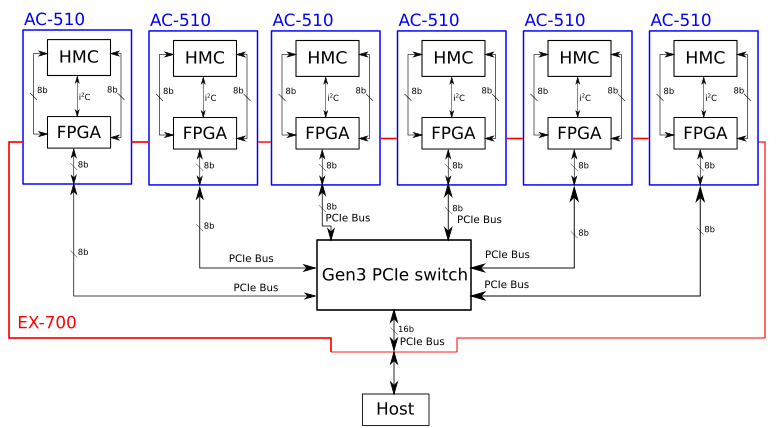
\includegraphics[scale = 0.4]{Figures/pico_board.png}
    \caption{Bloc Diagram of the Board}
    \label{fig:board_schema}
\end{figure}

\begin{minipage}[t]{0.6\textwidth}
\begin{figure}[H]
  \hspace{-15mm}  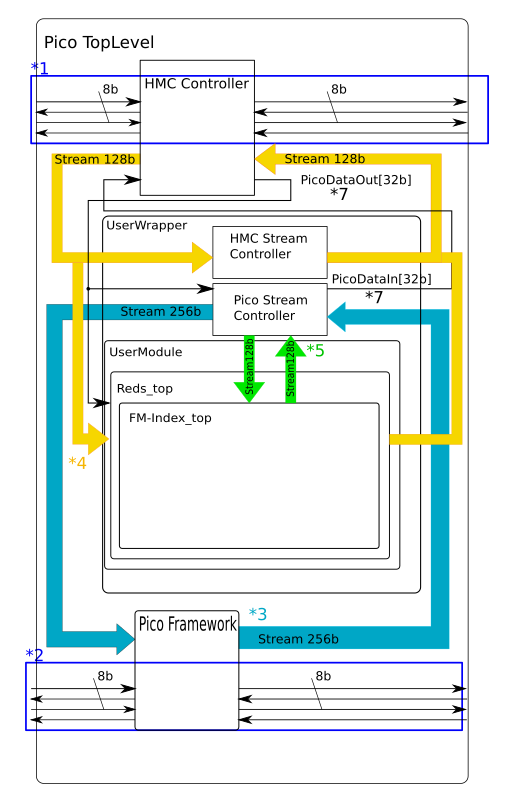
\includegraphics[scale = 0.6]{Figures/block_diagram.png}
    \caption{Bloc Diagram of the whole project}
    \label{fig:block_diag}
\end{figure}
\end{minipage}
\begin{minipage}[t]{0.35\textwidth}
Below are defined the differents references places on the Figures \ref{fig:block_diag} :
\begin{description}
\item [1] PCIe bus interface around the HMC controller, different from the \textrm{128-bit} wide bus used internally
\item [2] 8 parallel PCIe serial bus' for the \textsl{Pico Framework}, directly accessible from the host.
\item [3] Internal \textrm{256-bit} wide bus used to communicate with the lower-level design and the HMC.
\item [4] Internal \textrm{128-bit} wide bus used to communicate with the lower-level entity designed in this project and the \textsl{PicoBus}
\item [5] Internal \textrm{128-bit} wide bus used to communicate between the lower-level design and upper-level entities (e.g. host)
\item [6] \textrm{32-bit} wide direct bus between the \textsl{HMC Controller} and the lower-level entity designed in this project.
\end{description}
\end{minipage}

\section{Integration into the Vivado Project}

\begin{figure}
    \centering
    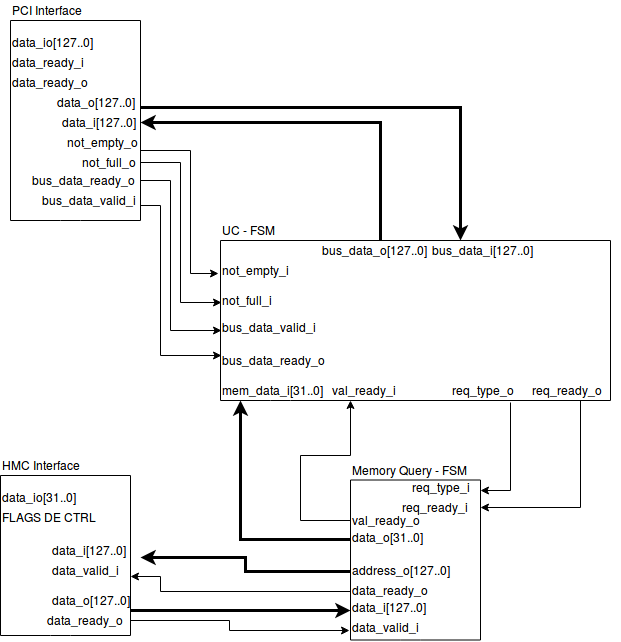
\includegraphics[scale = 0.5]{Figures/schema_bloc.png}
    \caption{FAIRE UN JOLI COMME LAUTRE}
    \label{fig:my_label}
\end{figure}

\subsection{Additional Blocs}

\begin{description}
\item [PCI Interface] - This bloc is the interface between the \textsl{PCI Express Bus} and the FM-Index bloc. It receives short reads and command from a master. In this interface, the FM-Index bloc is a slave, that wait for commands and data to start working. A FIFO is already implemented and this bloc consumes what is put into it. When a result is ready, it is placed in another FIFO that can be accessed by the computer master on the other end.
\item [HMC Interface] - Similarly to the previous bloc, this one is the interface between the board main memory and the FM-Index bloc. Only accessed through the \textsl{Memory Query} bloc, it is used to query data, may it be checkpoints entries, BWT entries of Sampled Suffix array elements. All transactions are 128bits wide and the interpretation of the received data in the \textsl{Memory Query} bloc.
\item [Memory Query] - This bloc is used by the FM-Index to issue all the different queries it might need along the string matching process, which means it implements all 3 "functions" needed by the FM-Index : $Occ$, $Count$ (thus $LF$) and $Walk-Left$ (with the sampled suffix array). Those queries can be about "checkpoints", BWT symbol or sampled suffix array entries and the type of said requests is specified by the \textrm{req\_type} signal. This bloc is then responsible for interpreting the received data and transmitting it in the appropriate form to the FM-Index bloc. Note that in the actual implementation, this bloc is part og the HMC Interface bloc.
\end{description}

\subsection{RED\_Top}

\begin{figure}[H]
    \centering
    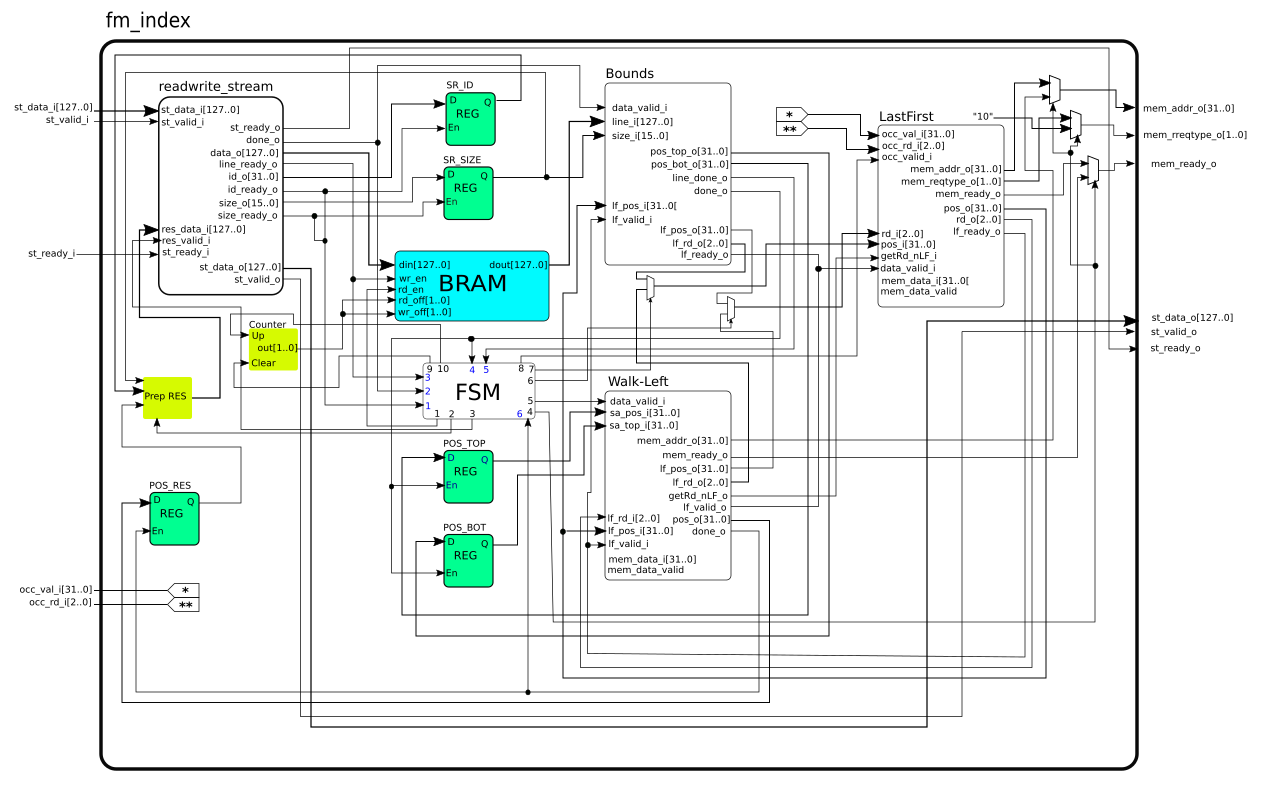
\includegraphics[scale = 0.4]{Figures/fmindex_top.png}
    \caption{FAIRE POUR REDS TOP Bloc Diagram of reds\_top}
    \label{fig:my_label}
\end{figure}

\subsection{PCI Interface}

SCHEMA BLOC, FSM

\subsection{HMC Interface}

SCHEMA BLOC, FSM, DIRE QUIL INCLU LA MEMQUERY

\subsection{Timing Requirements}

Inherited from the project are the timing requirements for the system, set at 250MHz, meaning that in order to produce a bitmap for the FPGA that would be guaranteed to behave as written, there should be no paths longer than 4 ns for a signal between two storing elements or port. \\
Considering the global structure of the implemented system, most paths respect this constraint as most exchanged data are stored into local registers and most operations are simple.\\

Nonetheless, the HMC Interface bloc had a path that did not last under that 4 ns, this being due to a rather unpleasant but necessary operation done one the position provided by the FM-Index. In the case of a query for a symbol of the BWT, the actual address is calculated by dividing this position by the number of symbol contained in each row, meaning here the inconvenient number 42. This kind of division is synthesized into a series of numerous simpler operations (see Fig. \ref{fig:timing}) with by default no storage element in between, thus creating a long path upon which we have little to no control. \\

\begin{figure}[H]
    \centering
    \hspace*{-3mm}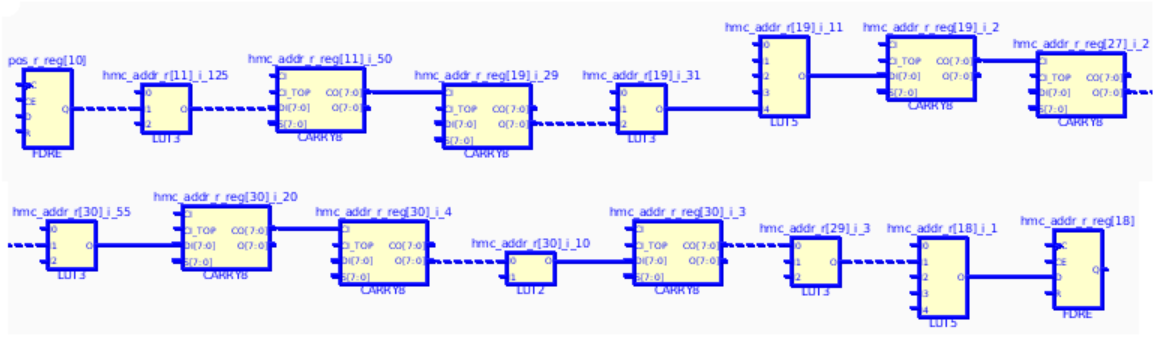
\includegraphics[scale = 0.4]{Figures/TIMING_RTL.png}
    \caption{RTL View of the hardware path generated}
    \label{fig:timing}
\end{figure}

After some digging [REFORMULER] it was enough to enable more control to the synthesizer on the timings and optimization of those kind of delays to reduce this time to just under 4 ns. 

Another solution would have been to simplify the problematic operation by encoding the BWT on 4 bits. This would have allowed 32 elements per memory row, and thus reducing the division to a simple 5-bit shift to the right in order to determine an element's row and its position in it. However, this would have increase the space needed to store 

\section{C++ Interface Implementation}

\subsection{Pico Framework}

\section{Co-Simulation}

\section{On-Board Testing}

\section{Validation}
